\documentclass[tikz,border=4pt]{standalone}
\usepackage{amsmath}
\begin{document}
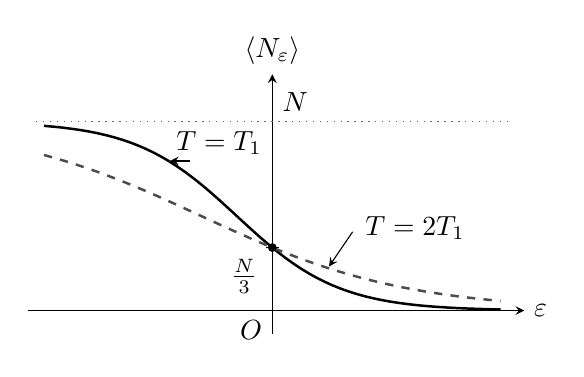
\begin{tikzpicture}[>=stealth, thick, scale=1.0]
  % Axes
  \draw[->, line width=0.4pt] (-3.1, 0) -- (3.2, 0) node[right] {$\varepsilon$};
  \draw[->, line width=0.4pt] (0, -0.3) -- (0, 3.0) node[above] {$\langle N_\varepsilon \rangle$};
  \node[below left] at (0, 0) {$O$};

  % Horizontal asymptote y = N (at y = 2.4)
  \draw[dotted, line width=0.5pt, black!60] (-3.0, 2.4) -- (3.0, 2.4);
  \node[above right] at (0, 2.4) {$N$};

  % Mark y = N/3 (at y = 0.8), label placed cleanly below-left away from dashed curve
  \draw[line width=0.4pt] (0.08, 0.8) -- (-0.08, 0.8);
  \node[below left] at (-0.06, 0.78) {$\frac{N}{3}$};

  % T = T1 (solid): N / (2*exp(x/0.65) + 1)
  \draw[line width=0.9pt, domain=-2.9:2.9, samples=120]
    plot (\x, {2.4 / (2 * exp(\x / 0.65) + 1)});

  % T = 2 T1 (dashed): N / (2*exp(x/1.3) + 1)
  \draw[dashed, line width=0.9pt, black!70, domain=-2.9:2.9, samples=120]
    plot (\x, {2.4 / (2 * exp(\x / 1.3) + 1)});

  % Intersection point (0, N/3)
  \fill (0, 0.8) circle (1.6pt);

  % Labels in open spaces
  \node[above right] at (-1.35, 1.85) {$T = T_1$};
  \draw[->, line width=0.4pt] (-1.05, 1.90) -- (-1.30, 1.90);

  \node[right] at (1.05, 1.05) {$T = 2T_1$};
  \draw[->, line width=0.4pt] (1.02, 1.0) -- (0.72, 0.56);
\end{tikzpicture}
\end{document}
